\chapter{The proposed automatic pitch correction system: technical presentation}
\label{chap:thesis-autotuner}
In this chapter, I describe the proposed system\cite{wager2020deep}. I start by discussing related work in pitch correction. Given that not much work has been done on the topic, I consider work on similar tasks such pitch detection, and relevant techniques in the broader fields of deep learning and signal processing. I then describe in detail the structure of the neural network, the data preparation steps---including de-tuning and feature extraction, the training configuration, and the experimental setup. 

%Introduction
%- based on chapters 2 and 3 (ok)
%- empirical (ok)
%- data-driven (ok)
%- applies to any culture it is trained on (ok)
%- overview

\section{Overview}
The system introduced in this thesis takes a data-driven approach to automatic pitch correction of solo singing performances. The proposed approach predicts note-wise pitch shifts from the relationship between the respective spectrograms of the singing and backing track. It outputs the amount and direction of the pitch shift expected to bring the note back in tune. In post-processing, it globally shifts each note by the predicted pitch shift. It does not require access to the musical score, which makes it usable even when the singer improvises or harmonizes in a performance.

I begin by illustrating the complexity of the task automatic pitch correction using the difference between a musical score and a performance. In a musical score, a melody for singing voice is typically notated as sequence of notes of discretized lengths and pre-defined pitches. The simplicity of the symbolic representation leaves considerable scope for variation in the singer's interpretation. Even when a vocalist follows the general contour of the score, the singing voice actually varies continuously due to expressive gestures such as pitch bending, vibrato, and any other variations coming from genre, personal preference, and random variation. The proposed data-driven approach tries to respect the nuanced variations of sung pitch, while the also actively estimating the amount of unintended pitch shift (see Fig. \ref{fig:results}).

\begin{figure}[t]
    \centering
    \includegraphics[width=\columnwidth]{figures/results.pdf}
    \caption{An example of the behavior of the proposed system. The red line shows the pitch contour of the vocal track input to the model. The green line shows the pitch contour after applying corrections predicted by the system. This plot shows a synthesized training example: The black line shows the original vocal track pitch contour, which was de-tuned to the red line to generate an input-target pair for supervised training.}
    \label{fig:results}
\end{figure}

The proposed system is designed to utilize similar information as the human ear, basing corrections on information found in the audio, such as the level of perceived musical harmony and context in time. It is a neural network trained on patterns in real-world singing examples using a dataset of 4,702 amateur karaoke performances selected for good intonation. The model is trained on both incorrect intonation, for which it learns a correction, and intentional pitch variation, which it learns to preserve. This approach differs from commercial systems such as Antares Auto-Tune, where vocal track notes are usually shifted to be centered around pitches in a user-defined score, or mapped to the closest pitch among the twelve equal-tempered scale degrees. The proposed system treats pitch as a continuous value rather than relying on a set of discretized values found in musical scales. The design of the proposed system is based on the empirically derived conceptualization of musical intonation described in Section \ref{sec:empirical}. Given its flexibility and preservation of nuance, it can be adapted to work for different musical cultures. It is a step towards a model-free automatic pitch correction system, the use of which is justified in Chapter \ref{chap:tech-background}. 

The proposed deep neural network consists of convolutional layers for feature extraction followed by gated recurrent units for sequential processing. The system shows promising performance on the real-world score-free singing pitch correction task. To the best of my knowledge, the proposed method is the first data-driven approach to correcting singing voice pitch based on its harmonic alignment to the backing track.

\section{Open-source repository}
%- code is available
An implementation of the system Python and Pytorch is available to the public at \url{https://github.com/sannawag/autotuner}\footnote{Note that the system used to be named \textit{Deep Autotuner}, but I have modified the name when possible to avoid confusion with the trademarked term \textit{Auto-Tune} by Antares}. Users have the option of training the model on their own dataset or of downloading the parameters of the model that provided the best test results. The repository also includes code for a baseline automatic pitch correction system introduced in \ref{sec:subjective-test}, and an implementation of the time-domain pitch-synchronous overlap and add (TD-PSOLA) algorithm \cite{charpentier1986diphone}. A standalone implementation of TD-PSOLA is available at \url{https://github.com/sannawag/TD-PSOLA}. The dataset used to train the model is available upon request via \url{https://ccrma.stanford.edu/damp}. Note that the CQT parameters used in the published version of the dataset are different from those referred to in this chapter.

\section{Related work}
%related work
%pitch correction
%- mention antares
The first commercial pitch-correction technique, Antares Auto-Tune \cite{antares:2016}, is also one of the most commonly used. Section \ref{sec:autotune} describes in detail how it works. Auto-Tune measures the fundamental frequency of the input monophonic singing recording, then re-synthesizes the pitch-corrected audio signal. In Auto-Tune and in recent work on continuous score-coded pitch correction \cite{salazar2015continuous}, each vocal note is pitch shifted to the nearest note in a user-input set of pitches (scale) or to the pitch in the score if it is known. The default musical scale is the equal-tempered scale, in which each pitch $p$ belongs to the set of MIDI pitches $[0, 1, ..., 127]$ and its frequency in Hertz is defined as $440*2^{\frac{p-69}{12}}$. Some users prefer a finer resolution and include more than twelve pitches per octave, or use intervals of varying sizes between pitches. In any case, the fundamental frequency is discretized to a small set of values, around which every note is shifted to be exactly centered. Hence, the pitch shifts tends to ignore a singer's intentional expressive gestures and might not easily apply to non-Western music with different scales or more fluidly varying pitch. The proposed system accommodates this variety of frequencies by letting the fundamental frequency take any value along a continuous scale, and by shifting every note by a constant without modifying internal pitch variation.

%- other pitch correction programs
Recent style-transfer-based work modifies amateur performances to mimic a professional-level performance of the same song. Luo \textit{et al.} proposed to match the pitch contour of the professional-level performance while preserving the spectral envelope of the amateur performance \cite{luo2018singing}. Meanwhile, Yong and Nam proposed to match both the pitch and amplitude envelopes \cite{yong2018singing}. Our model is similar in the sense that it also uses features gathered from high-quality performances \cite{wager2018intonation}. However, the proposed model does not necessitate a ``target" performance of the same song during testing. Instead, it learns from many in-tune singing voice examples and their backing tracks, and then generalizes to unknown songs, while preserving the original singer's style.

\subsection{Music information retrieval}
%pitch detection
%    - pitch detection (ok)
%    - CQT (ok)
Music Information Retrieval (MIR) research on related tasks such as pitch detection provides a useful background for this thesis. Gomez {\it et al.}\cite{gomez2018deep} provide an overview of recent developments in deep learning for singing processing, ranging from pitch detection to singing separation and synthesis. We focus here on pitch detection as it is particularly relevant to automatic pitch correction. It also aims to extract harmonic patterns from the audio, which correspond to perceived pitch. In the case of pitch detection, the perceived pitches are often manually annotated. 

Bittner \textit{et al.} introduce a fully convolutional DNN for polyphonic pitch transcription. The input is the magnitude harmonic constant-Q transform of the audio. The constant-Q transform (CQT) is a time-frequency transformation suitable for a convolutional neural network. It can be contrasted to the Fourier transform, which has linearly spaced center frequencies $f_n = n * \frac{SR}{N}$, where $n$ is the frequency bin index, $SR$ is the sampling rate, and $N$ is the dimension of the transformation space. The CQT instead has logarithmically spaced center frequencies $f_j = f_{min} * 2^{\frac{j}{b}}$ where $f_{min}$ is a pre-defined minimum frequency and $b$ determines the number of bins per octave. The fact that the center frequencies are logarithmically spaced results in the audio representation being translationally invariant, meaning that shifting a musical interval up or down will not change its spacing in the CQT. This enables a CNN filter to discover harmonic patterns across the full range of frequencies. Another advantage of the CQT representation is that it has a similar resolution to the human auditory system, with high resolution in the lower frequencies and wider bins in the higher frequencies. The downside of using CQT is that it cannot benefit from the Fast Fourier transform optimization, so is computationally expensive, $\mathcal{O}(N^2)$ instead of $\mathcal{O}(N \log (N))$. Bittner \textit{et al.} add more resolution by computing multiple, overlapping CQTs, each starting at a different frequency. This technique is called harmonic CQT (HCQT). The network structure includes four lower layers with small filters of dimension $5 \times 5$ or $3 \times 3$ to detect small-scale patterns. The fifth layer, instead, uses a filter that spans an octave of audio. This musically informed network design decision increases the relevant receptive field of each output state---the context in the input HCQT it can access---without needing to make the network very deep. The sixth layer then uses a $1 \times 1$ filter to combine all the learned features and output a pitch activation map. \cite{bittner2017deep} The DNN proposed in this thesis utilizes CNN layers whose structure is closely based on this network. Since our pitch correction task is sensitive even to a small amount of pitch shift, we also choose to use the CQT for its finer resolution in the lower frequencies. 

Basaran {\it et al.} add to the pitch detection CNN by adding a recurrent layer to incorporate the sequential nature of audio and music signals into their DNN structure. The network estimates the main melody in polyphonic audio signals in the constant-Q transform (CQT) representation, using a gated recurrent unit (GRU) layer \cite{chung2014empirical, ChoK2014arxiv} to model the temporal structures \cite{basaranmain}. 

\subsection{Deep learning}
%deep learning and audio
%    - Amazon paper for CNN + rnn structure + pre-training (ok)
Research in the larger fields of deep learning and audio signal processing also provides a useful background for the task. Wager \textit{et al.} improve the performance of a DNN with multiple layers by first training the lower layers on a smaller task, then initializing the corresponding the full network with the trained weights. The network---designed for automatic speech recognition---has a similar structure to the one proposed in this thesis, with linear lower layers for feature extraction followed by recurrent layers for sequential processing \cite{wager2020fully}.
%    - WaveNet
\textit{Wavenet} is a highly expressive model that can synthesize or transform sound at the level of the sample \cite{oord2016wavenet}. The \textit{Wavenet}-based dereverberation network introduced in \cite{su2020hifi} demonstrates that it is able to learn a transformation for a highly complex task. The network is trained in an adversarial manner \cite{goodfellow2014generative} to help the results retain the nature of the original signal. It provides inspiration for moving to a sample-by-sample model. Though this thesis does not include experiments using such a model, the concept of moving to a more fine-grained representation is compelling.

\subsection{Audio signal processing}
%pitch shifting
Monophonic pitch detection and transposition techniques provide tools for feature extraction and post-processing. The probabilistic YIN algorithm (pYIN) \cite{mauch2014pyin} is used as a benchmark for measuring frequency in monophonic music signals \cite{devaney2020new}. Unlike other state-of-the-art algoritms, including CREPE \cite{kim2018crepe}, its resolution is not limited to a margin such as 20 cents. While this precision is suitable for MIR tasks such as music recommendations, in the case of musical intonation, 20 cents can make the difference between being in tune or out of tune. the pYIN algorithm, like the pitch detection algorithm used for Antares Auto-Tune, is based on autocorrelation for periodicity detection. Autocorrelation alone is not always reliable: It might find a stronger periodicity at a harmonic---for example, the octave---or choose a maximum periodicity at value 0, when the signal is not shifted. The pYIN algorithm is based on the YIN pitch detection algorithm \cite{de2002yin}, which adds steps to autocorrelation to reduce error from 10\% to 0.5\%. These steps include a weighting of the autocorrelation output to reduce periodicity at harmonics, and a cumulative normalization that discourages selection of the 0-lag periodicity without a need for an arbitrary threshold. It also includes linear interpolation to further refine the pitch estimate. The pYIN algorithm applies a hidden Markov model (HMM) to the output of YIN, using a set of candidate periodicities instead of selecting the maximum one. This results in a smoother output. Both YIN and pYIN output 0 when they do not detect a period, making the output suitable for voice activity detection and note boundary analysis. The precision of the pitch measurement combined with the voice activity detection make pYIN ideal for the automatic pitch correction task. As described in \ref{sec:addthis}, the HMM used in pYIN inspires the HMM proposed in this thesis for detecting note boundaries. 

%- PSOLA: TD-PSOLA algorithm 
Another useful tool is TD-PSOLA, the time-domain pitch-synchronous overlap add algorithm for pitch shifting \cite{charpentier1986diphone}. Similarly to YIN, it starts by detecting periodicity in audio. It then splits the audio signal into individual periods, and shifts them slightly in time to produce the effect of shorter or longer periods. It uses cross-fading to avoid clipping. TD-PSOLA is suitable for the task because it produces a natural sounding result. Unlike other pitch-shifting techniques such as resampling, it does not modify the structure of the waveform except at the edges. This minimizes changes to the formant---the harmonic structure of the sound---so that the timbre is not modified along with the pitch. 
% probabilistic YIN --> also inspires own approach to HMM note parsing

\begin{figure*}[t]
\subfigure[]{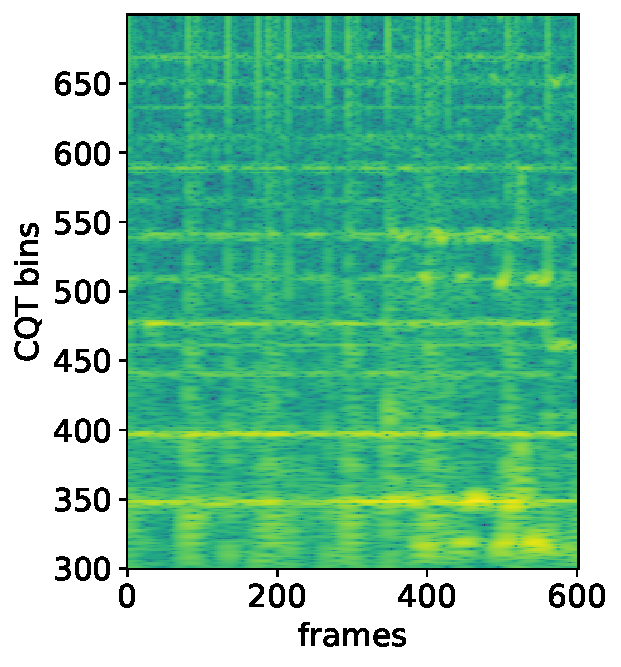
\includegraphics[height=1.625in]{figures/cqt_comparison_1.pdf}}\hspace{-.15in}%\vspace{-.03in}
\subfigure[]{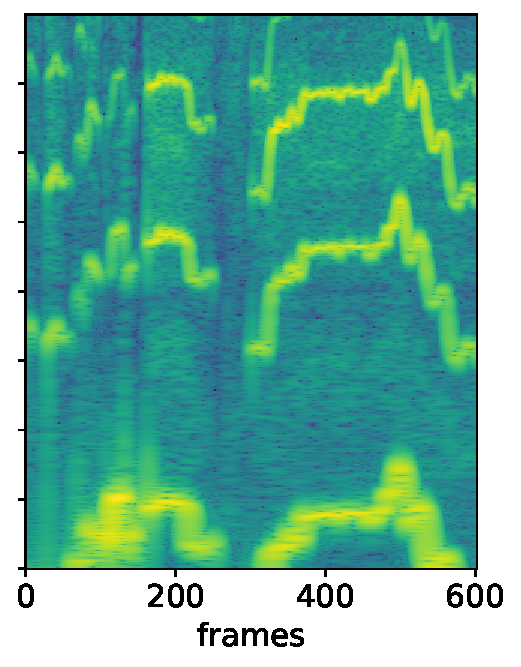
\includegraphics[height=1.625in]{figures/cqt_comparison_2.pdf}}\hspace{-.15in}%\vspace{-.03in}
\subfigure[]{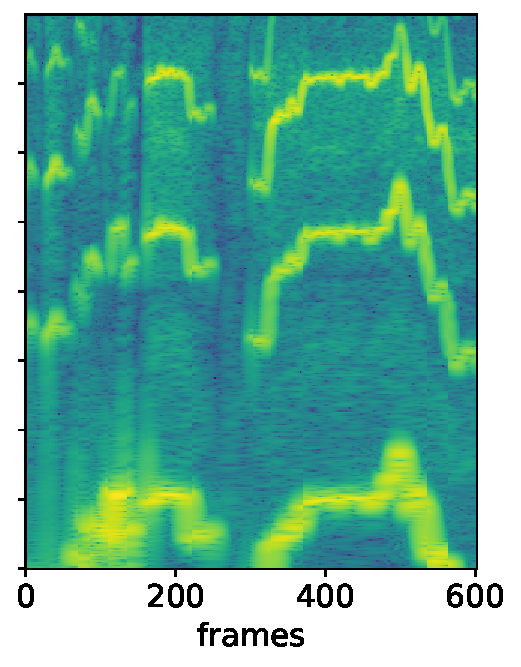
\includegraphics[height=1.625in]{figures/cqt_comparison_3.pdf}}\hspace{-.15in}%\vspace{-.03in}
\subfigure[]{\includegraphics[height=1.625in]{figures/cqt_comparison_4-2.pdf}}\hspace{-.15in}%\vspace{-.03in}
\subfigure[]{\includegraphics[height=1.625in]{figures/cqt_comparison_5-2.pdf}}\hspace{-.15in}%\vspace{-.03in}
    \caption{
    Constant-Q transform of the vocals and backing tracks computed using Librosa \cite{mcfee2015librosa}. We zoom into frequency bins 300 through 700 out of 1024 for better visibility. (a) shows the CQT of the backing track. The horizontal lines are due to constant pitches. (b) and (c) show the CQT of the vocals before and after the correction, respectively. (d) and (e) show the superposed vocals and backing track before and after corrections. The CQTs are binarized by the mean of their amplitude, which makes the louder components stand out for visibility (see Section \ref{sec:data-format-autotune}). In this example, we see that the correction shifted the pitch of the vocals up and centered it around the desired harmonics of the backing track (red circles).
    }
    \label{fig:model-input-autotune}
\end{figure*}

%Proposed model
\section{The proposed system}
\label{sec:proposed-autotune}
%- harmonic alignment (ok)
The proposed model predicts pitch correction based the CQT of the monophonic vocals and the backing track. Its structure is built on the assumption that the backing track has clearly identifiable pitches---a chord progression---which serves as a reference for the vocals. The program can then use the harmonic alignment between the vocals and backing tracks to make its predictions. Figure \ref{fig:model-input-autotune} shows the CQT of vocals and backing track excerpts of a few notes before and after applying predicted pitch corrections. In the excerpt, the backing track pitches are mostly constant, meaning that a chord is likely being held. After the correction, the vocals appear to be more closely aligned with the backing track, as can be seen in a CQT combining the two tracks. The shifts are subtle enough that they are difficult to see in the separate tracks. 

%- supervised training pairs. discuss this in data sec. (ok)
The model is trained in a supervised manner. Training data consists of pairs of performances that are identical except for the vocals pitch. The backing track remains fixed, as it is when the singer performs in a karaoke setting. The input-target pairs, while required to train the model, are difficult to come across naturally. Hence, I synthesize them by detuning high-quality singing performances to construct the input signals, and then train our model to predict the shifts that recover the original pitches. Section \ref{sec:data-format-autotune} describes the de-tuning process.
%    - applies to any culture it is trained on
%- time-frequency representation overview
%    - CQT

%- note splitting
%    - Discretization for control, constant shift
\subsection{Note-by-note processing}
\label{sec:notes}
A second strong assumption behind the proposed system design is that a singer targets a specific frequency per note, around which all pitch variations are centered. Given this assumption, the network corrects the pitch of one note by shifting all frames included in it by a constant. The first step to processing the song note by note is to detect the note boundaries from the original singing performance. I choose not to use a musical score, first, because this makes the program usable in the many situations where no score is available, second, because this avoids inconsistent note boundaries due to alignment errors or improvisation. Multiple approaches exist for score-free detection note boundaries: I investigated three. Their respective outputs can be visualized in Figure \ref{fig:note-parsing}.

\begin{figure}[t]
    \centering
    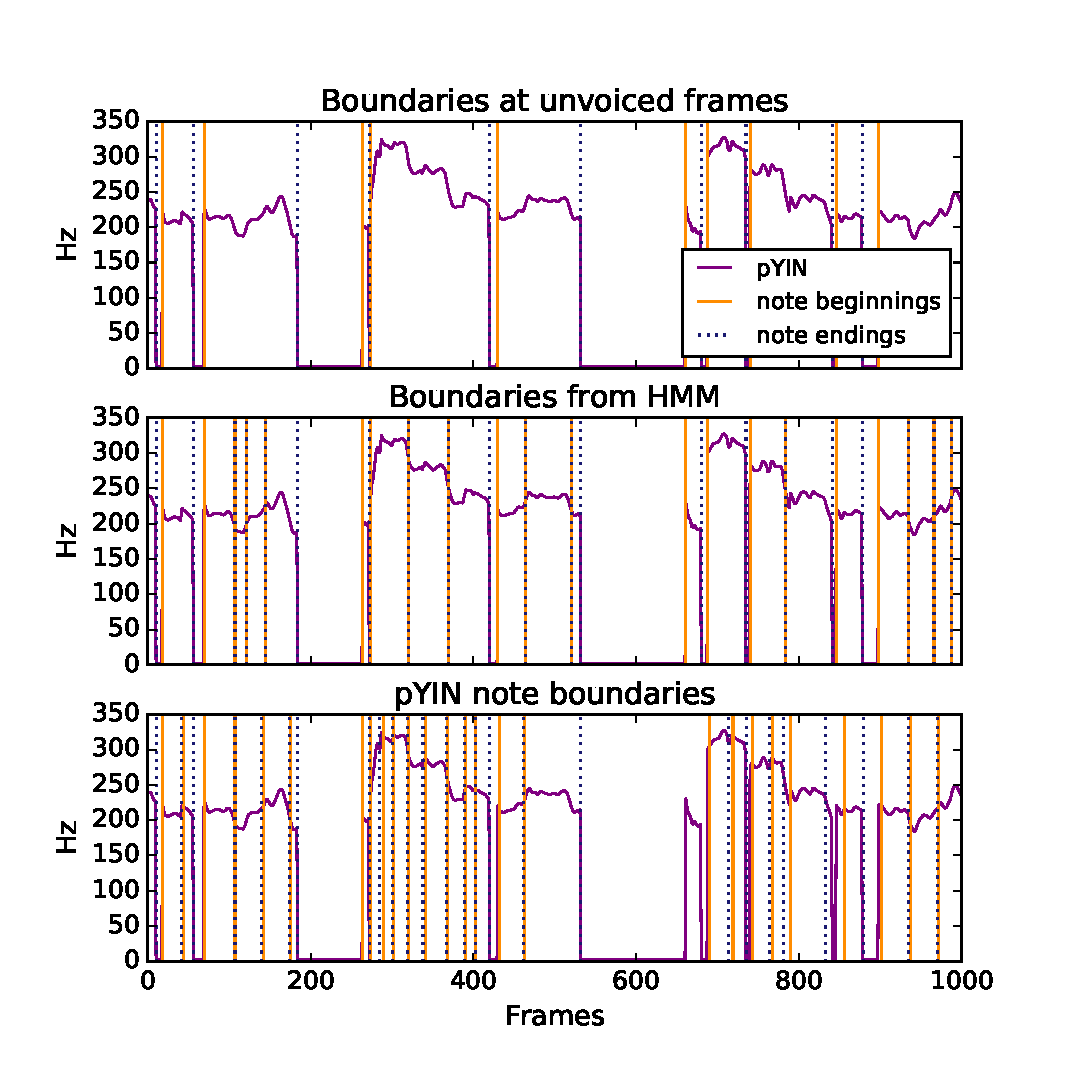
\includegraphics[width=\columnwidth]{figures/note_parse_comparison_attention_5.eps}
    \caption{Comparison of three different note boundary detection outputs for an excerpt from \textit{Attention} by Charlie Puth. The purple line shows the pYIN frame-wise pitch contour. The vertical lines show the note boundaries. The first and second approaches use the frame-wise pYIN pitch output. The first approach assigns note boundaries at the beginnings and ends of unvoiced sections. The second approach fits a Gaussian HMM to the pitch contour, and uses the hidden state sequence of equal-tempered scale frequencies along with unvoiced frames to assign boundaries. The third one uses the pYIN note-wise output. In this example, the unvoiced frame approach fails to split some legato passages into individual notes and the pYIN note approach is the most sensitive, assigning the largest number of notes. Sometimes this is musically relevant: for example, the lyrics in the three-step descending sequence around frames 300 to 400 are ``knew-that-I, knew-that-I, knew-that-I'', splitting each step into three musical events. The pYIN note detection detects these boundaries. However, it misses some notes---for example, the first note after frame 600---and its boundaries are not exactly aligned with the frames that switch between being voiced and unvoiced---for example, in multiple locations between frames 800 and 900.}
    \label{fig:note-parsing}
\end{figure}

The first, which I ended up choosing, was to define every transition silence as a note boundary. To this end, I analyzed the vocals pitch using the frame-wise probabilistic YIN (pYIN) algorithm \cite{mauch2014pyin}, implemented as a Vamp plugin in \cite{cannam2010sonic}. The frame-wise pitch is set to 0 for unvoiced frames, which makes it possible to easily treat transitions between voiced and unvoiced frames as note boundaries. A small amount of smoothing was required to avoid glitches in the case where a single frame had value 0. The advantage of this technique is that it minimizes artifacts during shifting. Any discontinuities arising due to pitch shifting a section of an audio recording are insignificant because the audio is silent at the discontinuity points. The disadvantage is that this note parsing technique fails to split notes when they are connected, though this is common in \textit{legato} melodies. This means that if one part of a legato passage is out of tune and another part isn't, a shift that would correct the out-of-tune part would de-tune the other part.

The second approach, which turned out to be too error-prone for the task of automatic pitch correction, was to use the note-wise pYIN plugin available as an extension to the original frame-level pitch detection algorithm algorithm. This program is useful for melody detection, but I found that it did not always start and end notes at exactly the right frame for minimizing discontinuity. It often left small gaps between the end of one note and the beginning of the next one, making it difficult to determine what to do with these unaccounted frames. It also tended to be rather sensitive, converting pitch bending into two discrete notes. Any undesirable splitting of notes can have a significant impact on the ability of the model to perform reliably well. If a part of a note is separated from the rest and shifted in a different direction, the unnatural result can be displeasing enough to make a whole excerpt sound bad to the listeners.

The third approach assigns note boundaries to the vocal track using a Gaussian HMM applied to the frame-wise pYIN pitch contour. This approach combines the reliable output of pYIN with a customized note parsing technique. The hidden states in the HMM are the equal-tempered scale frequencies within the range of the minimum and maximum value in the pitch contour, $440 * 2^{\frac{p - 69}{12}}$, where $p \in [21, 108]$, the standard MIDI range. They also include 0 for silence or unvoiced frames. The standard deviations correspond to the absolute difference in pitch between each equal-tempered scale frequency, leaving much room for the frame-wise pitch to deviate from the scale. The transition matrix is set to 0.001 everywhere except in the diagonal, which makes each row sum to 1. The starting probabilities are uniformly distributed. Fitting this model assigns a \textit{note} state to each frame and provides boundaries both between \textit{legato} notes and between unvoiced and voiced sections. The potential shortcoming of this approach is that it relies on the definition of a discretized scale. I note that it would be possible to use a more fine grained scale if working with a musical style that is not based on the equal-tempered scale---for example, use 22 subdivision of the octave for Classical Indian music. I used the equal-tempered scale here because the dataset I worked with was mostly made of popular music that used that scale.  

%    - hmm for note splitting (ok)
%        - now set up for equal-tempered for simplicity (ok)
%        - could set up a fine-grained scale, 22 notes as %in raga, or any other customization (ok)
% could, in the future, try WaveNet (ok)
%- model structure with CNN and RNN
\subsection{Neural network structure}
This section describes two versions of the proposed system. The second version is an extension of the first, designed to include more temporal context across notes. The first version of the network consists of six stacked convolutional layers followed by a GRU layer. The last output of the GRU is fed to a dense layer that predicts a single scalar output, the note-level pitch shift. The convolutional filters pre-process the spectrogram tensor, reducing its dimensionality while also learning abstract features. Next, the GRU---from which the network only uses the last output---reduces the representation of a variable-length note to a fixed-length vector. Finally, the dense layer predicts the pitch shift in the approximate range of $-1$ to $1$, which is mapped to a semitone in either direction, or $-100$ to $100$ cents. The activation after each convolutional layer is the rectified linear unit (ReLU) \cite{he2015delving}. There is no nonlinear activation after the final dense layer, as this might encourage nonzero values. One example is the hyperbolic tangent function, which tends to move values closer to $-1$ or $1$ and away from 0. 

The GRU recurrent structure is a way for the model to analyze the singer's note contour, which can last from a split second to multiple seconds, while smoothing over unvoiced or noisy sections. This is crucial because the algorithm is expected to rely on aligning harmonics, which only occur in pitched sounds. Another advantage of using the GRU is that the hidden state output by one note can initialize the hidden state for the following note, passing along some information about the previous notes. Even when using the simplest possible detuning model, which shifts every pitch by an independent amount, we can assume that some information from past notes (e.g. from the backing track) is useful.

\begin{table}[t]
  \begin{center}
    \caption{The proposed network architecture.}
    \begin{tabular}{|c||c|c|c|c|}
    \hline
      & Conv1 & Conv2 & Conv3 & Conv4 \\
      \hline
      \#Filters/Units & 128 & 64 & 64 & 64 \\
      Filter size & (5, 5) & (5, 5) & (3, 3) & (3, 3) \\
      Stride & (1, 2) & (1, 2) & (2, 2) & (1, 1) \\
      Padding & (2, 2) & (2, 2) & (1, 1) & (1, 1) \\
      \hline
      & Conv5 & Conv6 & GRU & FC \\
      \hline
      \#Filters/Units & 8 & 1 & 64 & 1 \\
      Filter size & (48, 1) & (1, 1) & & \\
      Stride & (1, 1) & (1, 1) & & \\
      Padding & (24, 1) & (0, 0) & & \\
      \hline
    \end{tabular}
    \vspace{-.1in}
    \label{tab:network}
  \end{center}
\end{table}

%- option of adding additional song-rnn
The second version of the system is designed to enable the model to include more temporal context. The final dense layer is replaced by a second GRU that takes as input the sequence of note representations output one-by-one by the first GRU. It finally applies a dense layer to the full sequence to output a song-level prediction sequence. This version has the potential to reach farther back in time, and include information from the chord progression in the backing track and long-term melodic patterns in the vocals. The downside of this model design is that the deep neural network is deeper, which makes it more difficult to train. 

% - predict shift, apply it later (ok)
Table \ref{tab:network} displays the structure of the proposed network without the song-level GRU extension. The feature extraction layers are convolutional, which is common for image processing. The input to the model is in spectrogram format, which resembles an image, except for the fact that its meaning is different along the time and frequency axes. In image progessing, dimensions reduction techniques like max pooling are common. These techniques treat the x and y axes in the same way, which we wish to avoid. To preserve the frequency patterns axis, we instead use strides of two only in the time axis in three of the convolutional layers, as done successfully for the task of learning latent representations for speech generation and transformation in \cite{hsu2017learning}. In the third layer, we also stride along the frequency axis, but perform this only once to not lose too much information. The fifth convolutional layer has a filter of size 48 in the frequency domain, which captures frequency relationships in a larger range of the CQT, as shown to be successful in \cite{bittner2017deep} and \cite{hsu2017learning}. 
The error function is the Mean-Squared Error (MSE) between the pitch shift estimate and ground truth over the full sequence of notes in a performance. The MSE corresponds to the error in cents using the formula $\left|\text{cent error}\right| = 100 * \sqrt{\text{MSE}}$. % When training and testing the program, MSE is the only objective accuracy metric, though we have audio examples for an informal evaluation. A subjective test provides a qualitative evaluation when applying automatic pitch correction to real-world singing examples.

\subsubsection{Applying the predicted pitch corrections}
Once the program has output pitch correction predictions, these are applied to the vocals. The TD-PSOLA algorithm provides a natural sounding output with few artifacts. The shifting is constant across note, and subtle cross-fading is applied between legato notes---in between which there is no silence---to avoid glitches at the boundaries.

%- post-processing focus
\subsection{Post-processing}
The neural network introduced in this thesis is not explicitly designed to work in real time. First, the system is designed for post-processing plug-ins such as are found in music apps like Smule. Second, the task of automatic pitch correction is challenging enough even given abundant computation time, so I choose to leave real-time applications to future work. 

Even in its current form, though, the model might be adaptable to near-real-time processing as it only uses information from previous notes to make a prediction for the current note. Even within a note, it processes one frame at a time in order. The challenge would be to make the data pre-processing---involving pitch detection and feature extraction---fast enough. 

%Dataset
%- Intonation introduction, refer to chapter (ok)
%    - genres in the dataset (ok)
%Real-world dataset (ok)
%- real-world set for testing (ok)
\subsection{Dataset}
\label{sec:dataset-autotune}
During my internship with Smule, Inc, a company that offers a singing app for smartphone, my team and I constructed a training dataset by deriving from the ``Intonation" dataset \cite{wager2018intonation}, which we assume to be a collection of in-tune singing voice tracks. A detailed description of the dataset, including instructions on how to access it, is available in Appendix \ref{chap:thesis-damp}. The 4702 separate vocal tracks in the dataset are mostly of Western popular music, collected by Smule for good intonation. While browsing the dataset, I also discovered a few tracks of Blues; Western Classical music; Latin, Japanese, and Indian popular music, country; and rock. I discuss this distribution in Appendix \ref{chap:thesis-damp}. While these real-world recordings contain some artifacts, no particular signal processing---e.g. denoising or filtering---has been applied to them. Each recording contains one minute of a performance, starting 30 seconds into the song. Although they are assumed to be in tune, this is not always exactly the case as the users are not necessarily professional singers. Overall, the sung pitch is sounds quite accurate and aligns reasonably well in timing and in pitch with the known musical score. Note when compared with the intended pitch. Hence, we can treat this paper as a proof of concept. The model can be trained on professional singing for best results.

Based on the metadata for each track indicating the backing track and user index, the dataset is split into 4561 training performances, 49 validation performances, and 64 test performances. The training set contains 709 backing tracks performed by 3468 different users, while the validation set is with 17 tracks sung by 43 users and the test set is with 16 sung by 62. There is no overlap in the backing tracks across the three sets. Overlap exists in the singer ID between the training and validation sets, but not with the test set. 

For a subjective listening test, I also create another real-world test set using the test backing tracks. Originally, 8 volunteers sang along with them outside of Smule. Singing experience ranged from beginner to semi-professional. The singers chose what to sing, and selected a total of 9 different arrangements. The dataset consisted of a total of 24 performances. The dataset later grew to N performances to increase its size and diversity of voices and singing styles. Instructions during the recording session included singing once in a normal manner and once mimicking an imaginary out-of-tune karaoke singer. The reason for this is that it is interesting to examine how the system performs both with performances that are already quite accurate, and with performances that are severely out of tune. Singers familiarized themselves with their chosen songs at their own pace over the course of a few days before the recording session. They used the Smule interface, which provides the lyrics and the piano roll score for reference. During the performance, they listened to the backing track through headphones so that it would not interfere with the vocals recording.

%De-tuning process
\subsection{The detuning process}
As introduced in Section \ref{sec:proposed-autotune}, the system is trained in a supervised manner. An input data sample consists of an out-of-tune performance, and the target consists of the note-wise shifts that should be applied to the vocals track to make it sound in tune. This type of pair is difficult to come across, unless one manually labels the corrections for every note in hundreds or in thousands of performances. The proposed approach to constructing training examples is to synthesize de-tuned examples. Singing performances from the ``Intonation'' dataset are de-tuned by shifting every note up or down and recording the amount of shift as the target. The synthetic pitch deviations are limited to approximately one semitone (100 cents) in either direction, a larger interval than the standard score-free approach of snapping to the nearest pitch, which limits the shift to 50 cents. In practice, it prevents errors in cases where the required shift is greater than 50, but can lead to degradation of the prediction accuracy on a too badly detuned input. 

To detune the training data, the program shifts the magnitude CQT up or down. This is expected to not produce too noticeable artifacts that the program could learn instead of the pitch relationships. The one issue is formant shifting, but this is not a big concern when only shifting by $\pm$100 cents or less. I experimented with shifting the training data using TD-PSOLA, but this did not produce noticeably better convergence, and increased the computational complexity due to the need to compute autocorrelation instead of simply shifting a matrix. 

\subsubsection{De-tuning distributions}
%- data de-tuning, different versions (ok)
%    - runif (ok)
%    - hmm (ok)
%        - MIR-1K (ok)
% rnn (ok)
The de-tuning process described in the previous section requires assigning a distribution to the random shifts. I experimented with two distributions. The first is the random uniform distribution in the range [-100, 100] cents, adjusted to the logarithmic scale of cents so that the shift of the CQT spectrogram is linear. Random uniformly distributed shifts are very simple to implement, and provide the model with plenty of examples of a wide variety of shifts, ranging from zero---which is useful, because singers are not likely to sing every note out of tune---to large ones. The downside is that this de-tuning technique is not based on real intonation patterns in out-of-tune singing. Furthermore, it is based on the strong and likely incorrect assumption that the detuning for every notes is independent from that of other notes.

A Gaussian HMM addresses both of the shortcomings of the random uniform distribution in a simple manner. HMM states represent deviation levels, while the Gaussian distribution provides variance. The HMM is trained on real-world singing examples in the publicly available MIR-1K dataset of karaoke performances \cite{su2009improvement}. The proposed HMM outputs deviations in cents from the equal-tempered scale. These deviations are represented as the difference between the equal-tempered frequency output by the HMM used to parse notes, described in Section \ref{ref:notes}, and the median of the measured frame-wide pYIN pitch. As before, the equal-tempered scale can be replaced with any other division of the octave. The proposed model uses five hidden states, but the number is arbitrarily chosen and can be replaced by a different value.  Sampling from this HMM produces sequences of pitch deviations that are based on real-world deviations and are not completely independent across notes.

To address the issue that all deviations will be 50 cents or less, because the distance to the nearest scale degree will never be greater than this, the MIDI pitch is moved by a semitone 5\% of the time across the median measured pitch, increasing the range to 100 cents. 5\% was another arbitrary choice, but the use of HMM is still expected to produce a slightly more accurate pitch behavior representation than the random uniform distribution.

The parameters learned from the MIR-1K dataset are in Table \ref{tab:detuning-hmm}. The means show a state very close to the equal-tempered scale, at 3, two that are offset by a few cents---one in each direction---and two that are more than a quarter tone away. We note that singers were very likely to start close to an equal-tempered scale degree, and almost never started far off. They also didn't tend to stay far off, as the transition probabilities from a larger deviation to a larger deviation are the smallest. We note that these parameters include the occasional shifts of the note across the median pitch.\footnote{I later realized that the pitch detection was based on mixed MIR-1K signals, which included the accompaniment. This resulted in a more spread distribution, but I believe this larger spread was useful for training the model to address larger shifts.}

\begin{table}[t]
  \begin{center}
    \begin{tabular}{|c|c|c|c|}
    \hline
      $\mu$ & $\sigma$ & $p_{start}$ & $p_{trans}$ \\
      \hline
      &&& \\
      $\left[ \begin{array}{c} 52 \\  13 \\3\\-8\\-73 \end{array}\right]$
      & $\left[ \begin{array}{c} 31  \\ 25\\16\\25\\24 \end{array}\right]$
      & $\left[ \begin{array}{c} 0.1  \\ 9\\76\\15\\0.1 \end{array}\right]$
      & $\left[ \begin{array}{ccccc} 4 & 30 & 30 & 35 & 1  \\ 13&27&30&24&5\\24&17&22&15&23\\16&25&28&23&7\\3&36&30&30&0 \end{array}\right]$  \\
      &&& \\
      \hline
    \end{tabular}
    \label{tab:detuning-hmm}
    \caption{The de-tuning Gaussian HMM parameters fitted to the MIR-1K dataset. The first column shows the means, or hidden states, and the second column shows the standard deviations. The final two columns show the start and transition probabilities. All parameters are in cents, a logarithmic measure, and rounded to the nearest integer, except for zeros, which are set to $0.1$ to show that no transition had zero probability}
  \end{center}
\end{table}

The HMM model pitch deviation is not the most complex model that could be used for the task. It could be replaced by a RNN that uses additional information, such as absolute frequency---given that a singer might be more likely to sing sharp or flat based on the register---or spectral information. One could go another step further and synthesize out-of-tune singing using a WaveNet and/or adversarial training.

\subsection{Data pre-processing details}
\label{sec:data-format-autotune}
The audio signals are normalized, then transformed using the CQT. The CQT covers 5.5 octaves with a resolution of 16 bins per semitone. The lowest frequency is 125 Hz. The top and bottom 16 bins are used as a buffer for pitch shifting, then truncated so that every input has dimension 1024. The frame size spans 92 ms and the hop size 11 ms. The vocals and backing track CQTs form two input channels to the neural network. In previous work, I experimented with using a third channel that would help bring out the contrast between the first two channels. I binarized the two CQT spectrograms using the mean modulus as a threshold, a technique used in computer vision \cite{sezgin2004survey}. I then took the bitwise disagreement of the two matrices based on the expectation that the in-tune singing voice, better aligned with the backing track, would cancel out more harmonic peaks than the out-of-tune tracks. Fig. \ref{fig:model-input-autotune} illustrates the three channels. It includes the binarized CQT before and after shifting though the third channel was ultimately left out, because it helps visualize the shift. Surprisingly, though the convergence with the third channel was better for multiple epochs, the loss with two channels ultimately dropped below its counterpart. The difference took long enough to appear that I only discovered it because I had forgotten to shut down the training for the two versions of the model after having already concluded that the third channel improved the results. 
%- CQT parameters, etc… (ok)
%- tried third channel, did not help (ok)
%- tried the binary channel but did not help (plot)? (ok)
%- Tried TD-PSOLA, expensive but not better (ok)

%Experimental setup
\section{Experimental configuration}
\label{sec:experiments-autotune}
\subsection{Training setup}
The program uses the Adam optimizer \cite{kingma2014adam}. It processes one note at a time as a minibatch of seven differently pitch-shifted versions. It does not include batch normalization because the different versions of the same note are not \textit{i.i.d}. When using the second GRU layer that bases the prediction on the sequence of notes, the outputs for each note are stored, then input to the GRU. 

The program applies gradient clipping \cite{pascanu2013difficulty} with a threshold of 100. It reports validation loss every 500 songs and save the model with the best result along with the latest one. 
%- loss function, etc… (ok)
%- Adam (ok)
\subsection{Initialization}
The convolutional parameters are initialized using He \cite{he2015delving}, and the GRU hidden state of the first note of every song is initialized using a normal distribution with $\mu=0$ and $sd=0.0001$. The hidden state of the note sequence GRU is initialized in the same way. When using the note sequence GRU, the weights from the note-by-note model can optionally be used to initialize the lower layers. These lower layers can also be ``frozen'' for some epochs before being trained in the context of the full model. 

\subsection{Experiments}
\label{sec:experiment-list}
In this thesis, I report test results on a set of different configurations, listed in Table \ref{table:experiments}. Note that I only report configurations that showed the strongest convergence. First, I compare note parsing techniques and de-tuning techniques when training the smaller version of the model. For the best performing models, I add the song-level GRU extension. I train the extended model either from scratch or initializing feature extraction parameters with the values learned for the smaller model. In the latter case, I freeze the pre-trained weights for one epoch. For each model, I report results either with learning rate 0.00001 or 0.000005, based on which setting converged best. Other learning rates did not converge.

\begin{table*}
\centering
\begin{tabularx}{\columnwidth}{ |X|X|X|X|X| } 
\hline
\multicolumn{5}{|c|}{\textbf{Experiment settings}}\\
\hline\hline
\textbf{Note parsing} & \textbf{De-tuning} & \textbf{Learning rate} & \textbf{Extension} & \textbf{Initialization} \\
\hline\hline
Silence & Uniform & 0.00001 & No & He, Gauss \\
\hline
Silence & HMM & 0.000005 & No & He, Gauss\\ 
\hline
HMM & HMM & 0.00001 & No & He, Gauss\\ 
\hline
Silence & Uniform & 0.000005 & Yes & pre-trained, Gauss\\
\hline
Silence & HMM & 0.000005 & Yes & He, Gauss\\ 
\hline
Silence & HMM & 0.000005 & Yes & pre-trained, Gauss\\ 
\hline
\end{tabularx}
\label{table:experiments}
\caption{The \textit{Note parsing} column indicates whether the note boundaries were assigned based on silent pYIN frames or based on state changes in the HMM assigning a scale degree to each frame. The \textit{De-tuning} column indicates whether the de-tuning distribution was random uniform or sampled from the HMM trained on MIR-1K. The \textit{Extension} refers to whether the song-level GRU is added to the model architecture. Finally, the \textit{Initialization} column provides the distributions used to initialize the parameters, and whether the feature extraction layers were initialized using pre-trained parameters from the model without extension.}
\end{table*}

%\begin{table*}
%\centering
%\begin{tabularx}{\columnwidth}{ |X|X|X|X| } 
%\hline
%\multicolumn{4}{|c|}{\textbf{Experiment settings}}\\
%\hline\hline
%\textbf{Model names} & \textbf{Learning rate} & \textbf{Initialization} & \textbf{De-tuning} \\
%\hline\hline
%Note-runif-1e-5 & 0.00001  & He, Gauss & Uniform \\
%\hline
%Note-runif-5e-6 & 0.000005 & He, Gauss & Uniform \\
%\hline
%Note-HMM-1e-5 & 0.00001 & He, Gauss & HMM \\ 
%\hline
%Song-runif-1e-5 &  0.00001 & He, Gauss & Uniform \\ 
%\hline
%Song-runif-5e-6 &  0.000005 & He, Gauss& Uniform \\ 
%\hline
%Song-HMM-1e-5 & 0.00001 & He, Gauss & HMM \\ 
%\hline
%Song-HMM-5e-6 & 0.000005 & He, Gauss & HMM \\ 
%\hline
%Song-HMM-pretrain-1e-5 & 0.00001 & ``Note-HMM-1e-5'' weights, Gauss & HMM \\ 
%\hline
%Song-runif-pretrain-1e-5 & 0.00001 & ``Note-HMM-1e-5'' weights, Gauss & Uniform\\
%\hline
%\end{tabularx}
%\label{table:experiments}
%\caption{List of experiments}
%\end{table*}

%- initialization of weights
%- pre-training
%Experiments
%- runif by note
%- hmm by note
%- runif by sequence
%- hmm by sequence
%- learning rates
%- + pre-training